\documentclass[12pt]{article}
\usepackage[margin=2.5cm]{geometry}
\usepackage{enumerate}
\usepackage{amsfonts}
\usepackage{amsmath}
\usepackage{fancyhdr}
\usepackage{amsmath}
\usepackage{amssymb}
\usepackage{amsthm}
\usepackage{mdframed}
\usepackage{graphicx}
\usepackage{subcaption}
\usepackage{adjustbox}
\usepackage{listings}
\usepackage{xcolor}
\usepackage{booktabs}
\usepackage[utf]{kotex}
\usepackage{hyperref}

\definecolor{codegreen}{rgb}{0,0.6,0}
\definecolor{codegray}{rgb}{0.5,0.5,0.5}
\definecolor{codepurple}{rgb}{0.58,0,0.82}
\definecolor{backcolour}{rgb}{0.95,0.95,0.92}

\lstdefinestyle{mystyle}{
    backgroundcolor=\color{backcolour},
    commentstyle=\color{codegreen},
    keywordstyle=\color{magenta},
    numberstyle=\tiny\color{codegray},
    stringstyle=\color{codepurple},
    basicstyle=\ttfamily\footnotesize,
    breakatwhitespace=false,
    breaklines=true,
    captionpos=b,
    keepspaces=true,
    numbers=left,
    numbersep=5pt,
    showspaces=false,
    showstringspaces=false,
    showtabs=false,
    tabsize=1
}

\lstset{style=mystyle}

\pagestyle{fancy}
\renewcommand{\headrulewidth}{0.4pt}
\lhead{Hyungmo Gu}
\rhead{CSC369 Week 6 Notes}

\begin{document}
\title{CSC369 Week 6 Notes}
\author{Hyungmo Gu}
\maketitle

\bigskip

\section{Virtual Memory \& Page Replacement}

\bigskip

\begin{itemize}
    \item Recap
    \begin{itemize}
        \item Solves \textbf{internal fragmentation} and \textbf{external fragmentation}
        \item Stores and retrieves data from \textbf{secondary storage} for use
        in \textbf{main memory} $^{[1]}$
        \begin{itemize}
            \item Secondary storage $\to$ Hard Drive
            \item Main memory $\to$ RAM
        \end{itemize}
        \item Is an important part of \textbf{virtual memory} management in modern
        OS $^{[1]}$
        \item Partitions memory into equal, fixed-size chunks
        \begin{itemize}
            \item Are called \textbf{page frames} or \textbf{frames}
        \end{itemize}
        \item Divide processes' memory into chunks of the same size
        \begin{itemize}
            \item These are called \textbf{pages}
        \end{itemize}
    \end{itemize}

    \begin{center}
    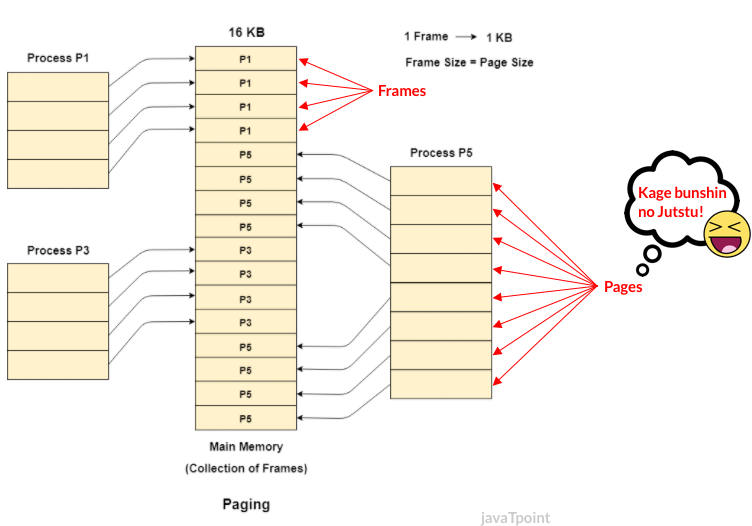
\includegraphics[width=0.8\linewidth]{../images/week_6_notes_1_1.png}
    \end{center}

    \bigskip

    \underline{\textbf{Refernces:}}

    \bigskip

    \begin{enumerate}[1)]
        \item Wikipedia: Paging, \href{https://en.wikipedia.org/wiki/Paging}{link}
        \item JavaTPoint: Paging with Example, \href{https://www.javatpoint.com/os-paging-with-example}{link}
    \end{enumerate}
    % \item Page Lookups Overview
    % \item TLBs
    % \item Summary so far: Paging
    \item Summary so far: Page Table
    \begin{itemize}
        \item Is the data structure used by a virtual memory system in computer
        operating system to store the mapping between virtual addresses and physical
        addresses.
    \end{itemize}

    \bigskip

    \begin{enumerate}[1)]
        \item Wikipedia: Page Table, \href{https://en.wikipedia.org/wiki/Page_table}{link}
    \end{enumerate}
    % \item How much space does a page table take up?
    % \item Managing Page Tables
    % \item Motivation: Two-Level Page Tables
    \item Multilevel Page Tables
    % \item Two-Level Page Tables
    % \item Two-Level Paging Example
    % \item Pentium Address Translation
    \item Inverted Page Tables (Read the book)
    \begin{itemize}
        \item Is an alternate to ever-increasing levels in page hierarchy $^{[1]}$
        \item Advantages $^{[1]}$
        \begin{itemize}
            \item Saves a lot of space (when the virtual address is much larger
            than the physical memory)
        \end{itemize}
        \item Disadvantages $^{[1]}$
        \begin{itemize}
            \item Increased difficulty of virtual to physical translation
        \end{itemize}
    \end{itemize}

    \bigskip

    \underline{\textbf{Refernces:}}

    \bigskip

    \begin{enumerate}[1)]
        \item Tanebaum AS, Boss H. 2015. Modern Operating Systems. 4th Edition. New Jersy: Pearson Education, Inc.
    \end{enumerate}
    % \item Efficient Translations
    % \item Page Allocation \& Eviction
    % \item Recap: Paging
    \item Page Faults
    % \item Policy Decision
    \item Demand Paging
    \item Prepaging (aka Prefetching)
    % \item Policy Decisions
    % \item Placement Policy
    % \item Policy Decisions
    % \item Evictng the Best Page
    \item Belady's Algorithm
    % \item What are possible Replacement Algorithms?
    \item Page Table Entries(PTE)
    \item Not-Recently-Used (NRU)
    \item First-In First-Out (FIFO)
    % \item Example of Belady's Anomaly
    \item Second-Chance
    % \item Implementing Second-Chance (clock)
    % \item Modeling Clock
    \item Least Recently Used (LRU)
    % \item Implementing Exact LRU
    % \item Modelling Exact LRU
    % \item Approximating LRU
    \item Counting-based Replacement
    % \item What are Possible Replacement Algorithms?
    % \item Fixed vs Variable Space
    % \item Working Set Model
    % \item Working Set Size
    % \item Working Set Problems
    \item Page Fault Frequench(PFF)
    \item Thrashing
    % \item Windows XP Paging Policy
    % \item Linux Paging
\end{itemize}

\end{document}